\documentclass{standalone}

\usepackage{tikz}

\usetikzlibrary{shapes, positioning}

\begin{document}

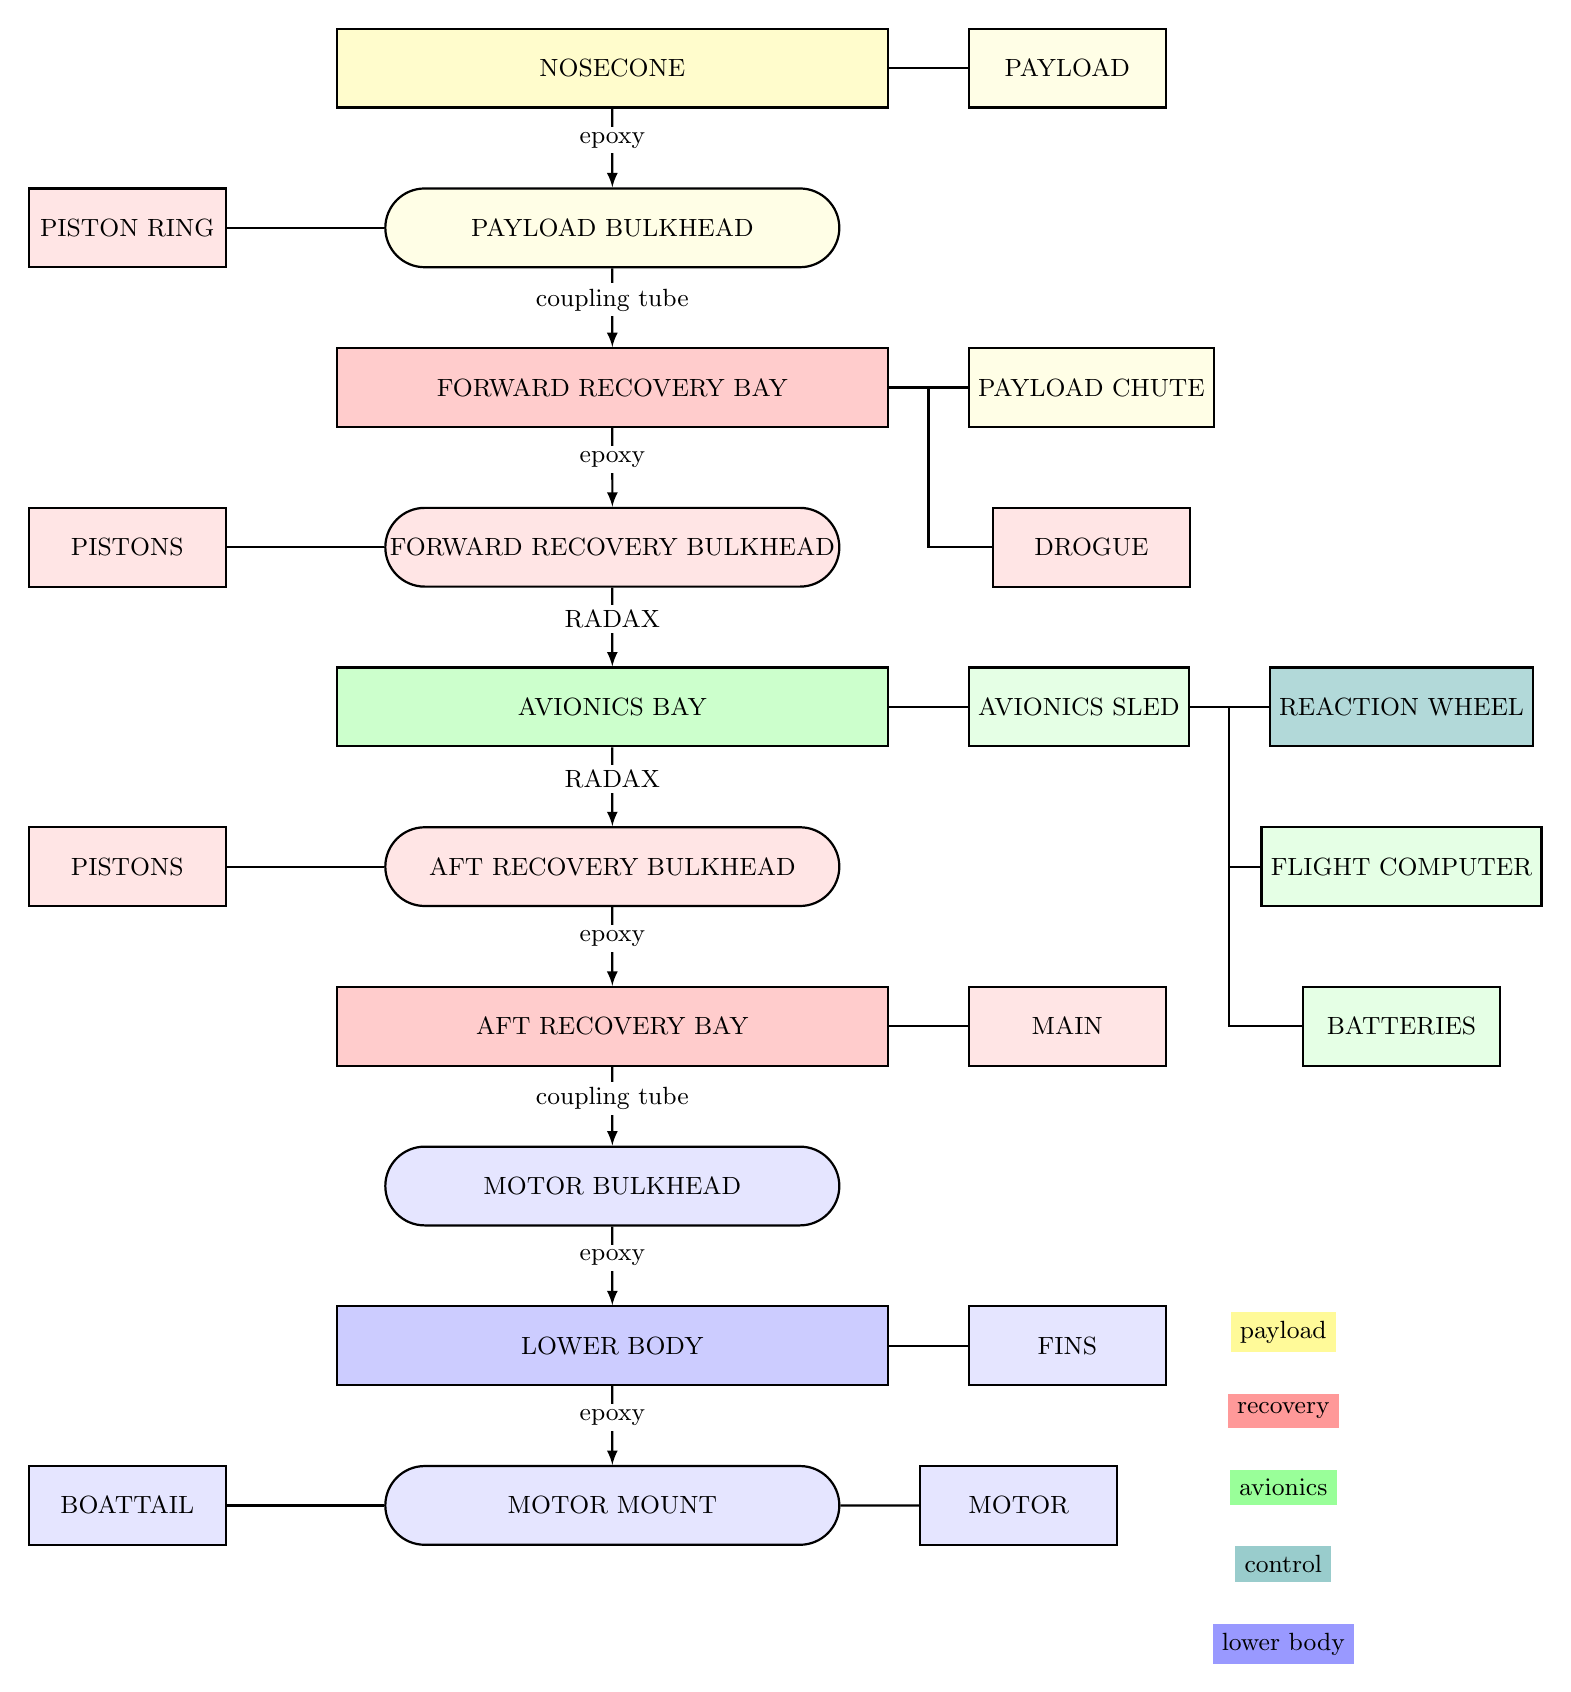
\begin{tikzpicture}[font=\small,thick];

% main line of boxes

\node[draw, fill=yellow!20, minimum width=7cm, minimum height=1cm] (nosecone) {NOSECONE};
\node[draw, fill=yellow!10, rounded rectangle, below = of nosecone, minimum width=6cm, minimum height=1cm] (pldbh) {PAYLOAD BULKHEAD};
\node[draw, fill=red!20, below = of pldbh, minimum width=7cm, minimum height=1cm] (fwdrecbay) {FORWARD RECOVERY BAY};
\node[draw, fill=red!10, rounded rectangle, below = of fwdrecbay, minimum width=6cm, minimum height=1cm] (fwdrecbh) {FORWARD RECOVERY BULKHEAD};
\node[draw, fill=green!20, below = of fwdrecbh, minimum width=7cm, minimum height=1cm] (avbay) {AVIONICS BAY};
\node[draw, fill=red!10, rounded rectangle, below = of avbay, minimum width=6cm, minimum height=1cm] (aftrecbh) {AFT RECOVERY BULKHEAD};
\node[draw, fill=red!20, below = of aftrecbh, minimum width=7cm, minimum height=1cm] (aftrecbay) {AFT RECOVERY BAY};
\node[draw, fill=blue!10, rounded rectangle, below = of aftrecbay, minimum width=6cm, minimum height=1cm] (motorbh) {MOTOR BULKHEAD};
\node[draw, fill=blue!20, below = of motorbh, minimum width=7cm, minimum height=1cm] (lowerbody) {LOWER BODY};
\node[draw, fill=blue!10, rounded rectangle, below = of lowerbody, minimum width=6cm, minimum height=1cm] (motormount) {MOTOR MOUNT};

% line to the right

\node[draw, fill=yellow!10, minimum width=2.5cm, minimum height=1cm, right=of nosecone] (payload) {PAYLOAD};
\node[draw, fill=red!10, minimum width=2.5cm, minimum height=1cm, left=2cm of pldbh ] (pistonring) {PISTON RING};
\node[draw, fill=yellow!10, minimum width=2.5cm, minimum height=1cm, right=of fwdrecbay] (pldchute) {PAYLOAD CHUTE};
\node[draw, fill=red!10, minimum width=2.5cm, minimum height=1cm, below = of pldchute] (drogue) {DROGUE};
\node[draw, fill=red!10, minimum width=2.5cm, minimum height=1cm, left=2cm of fwdrecbh ] (piston1) {PISTONS};
\node[draw, fill=green!10, minimum width=2.5cm, minimum height=1cm, right=of avbay] (avsled) {AVIONICS SLED};
\node[draw, fill=teal!30, minimum width=2.5cm, minimum height=1cm, right=of avsled] (rxnwheel) {REACTION WHEEL};
\node[draw, fill=green!10, minimum width=2.5cm, minimum height=1cm, below=of rxnwheel] (pcbs) {FLIGHT COMPUTER};
\node[draw, fill=green!10, minimum width=2.5cm, minimum height=1cm, below=of pcbs] (batts) {BATTERIES};
\node[draw, fill=red!10, minimum width=2.5cm, minimum height=1cm, left= 2cm of aftrecbh ] (piston2) {PISTONS};
%\node[draw, fill=teal!30, minimum width=2.5cm, minimum height=1cm, below=of piston2] (airbrakes) {AIRBRAKES};
\node[draw, fill=red!10, minimum width=2.5cm, minimum height=1cm, right=of aftrecbay] (mainchute) {MAIN};
\node[draw, fill=blue!10, minimum width=2.5cm, minimum height=1cm, right=of motormount] (motor) {MOTOR};
\node[draw, fill=blue!10, minimum width=2.5cm, minimum height=1cm, right=of lowerbody] (fins) {FINS};
\node[draw, fill=blue!10, minimum width=2.5cm, minimum height=1cm, left=2cm of motormount] (boattail) {BOATTAIL};
% arrows

\draw[-latex]
    (nosecone) edge node[pos=0.4, fill=white, inner sep=2pt]{epoxy} (pldbh)
    (pldbh) edge node[pos=0.4, fill=white, inner sep=2pt]{coupling tube} (fwdrecbay)
    (fwdrecbay) edge node[pos=0.4, fill=white, inner sep=2pt]{epoxy} (fwdrecbh)
    (fwdrecbh) edge node[pos=0.4, fill=white, inner sep=2pt]{RADAX} (avbay)
    (avbay) edge node[pos=0.4, fill=white, inner sep=2pt]{RADAX} (aftrecbh)
    (aftrecbh) edge node[pos=0.4, fill=white, inner sep=2pt]{epoxy} (aftrecbay)
    (aftrecbay) edge node[pos=0.4, fill=white, inner sep=2pt]{coupling tube} (motorbh)
    (motorbh) edge node[pos=0.4, fill=white, inner sep=2pt]{epoxy} (lowerbody)
    (lowerbody) edge node[pos=0.4, fill=white, inner sep=2pt]{epoxy} (motormount);


\draw (nosecone) edge (payload);
\draw (pldbh) edge (pistonring);
\draw (fwdrecbay) edge (pldchute);
\node [coordinate, right = 0.5 cm of fwdrecbay] (fwdrecpoint) {};
\draw (fwdrecpoint) |- (drogue);
\draw (fwdrecbh) edge (piston1);
\draw (avbay) edge (avsled);
\draw (avsled) edge (rxnwheel);
\node [coordinate, right = 0.5 cm of avsled] (avsledpoint) {};
\draw (avsledpoint) |- (pcbs);
\draw (avsledpoint) |- (batts);
\draw (aftrecbh) edge (piston2);
\node [coordinate, left=1.5 cm of aftrecbh] (aftrecpoint) {};
%\draw (aftrecpoint) |- (airbrakes);
\draw (aftrecbay) edge (mainchute);
\draw (motormount) edge (motor);
%\node [coordinate, right=0.5cm of lowerbody] (lowerbodypoint) {};
\draw (lowerbody) edge (fins);
\draw (motormount) edge (boattail);

% legend

\node[fill=yellow!40,above right=2cm of motor] (color1) {payload};
\node[fill=red!40, below=0.5cm of color1] (color2) {recovery};
\node[fill=green!40, below=0.5cm of color2] (color3) {avionics};
\node[fill=teal!40, below=0.5cm of color3] (color4) {control};
\node[fill=blue!40, below=0.5cm of color4] (color5) {lower body};


\end{tikzpicture}

\end{document}
